\documentclass{article}
\usepackage[top=1in, bottom=1in, left=1in, right=1in]{geometry}
\usepackage{amsmath}
\usepackage{graphicx}
\usepackage{subcaption}

\author{Jae Lee}
\title{Differential flatness control for multi-rotor in Gazebo simulation}

\begin{document}
\maketitle

\subsection*{Introduction}
Multirotor is one of the most popular platform in the beginning era of robotics. Its dynamics and control have been studied and developed to be stable and practical enough for easy use. It can perform many tasks that fixed-wing platform is not feasible due to its forward velocity constraint such as indoor navigation, aerial photography, and site inspection. In this paper, a control scheme called 'differential flatness control'(DFC) is introduced and applied to multirotor platform and LQR is used internally in this control scheme. First, DFC is prototyped in MATLAB and is verified that it is feasible. Second, ROS and Gazebo simulator are used to convince that DFC would work in hardware. Hardware implementation is not presented in this paper, but is left as future work.

\subsection*{Multi Rotor Dynamics}
The common states for multirotor dynamic model are composed of position, velocity, euler angles in inertial NED frame and angular velocity in multi rotor body frame. In this paper, simplified states are used and works without deteriorating result and they are position, velocity and yaw angle as shown below.

\[x=[p_n\ p_e\ p_d\ \dot{p_n}\ \dot{p_e}\ \dot{p_d}\ \psi]^T \tag{1} \label{eq1}\]

The input to multirotor state space model is as shown below.
\[u=\begin{bmatrix}
u_1 \\ u_2 \\ u_3 \\ u_4
\end{bmatrix}=\begin{bmatrix}
\ddot{p_n} \\ \ddot{p_e} \\ \ddot{p_d}-g \\ \dot{\psi}
\end{bmatrix} =\begin{bmatrix}
R_b^i(\psi,\theta,\phi)\begin{bmatrix}
0\\ 0\\ \frac{-T}{m}
\end{bmatrix} \\
q\frac{\sin\phi}{\cos\theta}+r\frac{\cos\phi}{\cos\theta}
\end{bmatrix} \tag{2} \label{eq2}\]
where g is gravity and m is the mass of multirotor.
From the states and input above, we can form complete state-space model.
\[\dot{x}=Ax+Bu+bg\]
where \[A=\begin{bmatrix}
0_{3x3} & I_{3x3} & 0_{3x1}\\
0_{3x3} & 0_{3x3} & 0_{3x1}\\
0_{1x3} & 0_{1x3} & 0_{1x1}
\end{bmatrix}, \ B=\begin{bmatrix}
0_{3x3} & 0_{3x1}\\
I_{3x3} & 0_{3x1}\\
0_{1x3} & 1
\end{bmatrix}, \ b=\begin{bmatrix}
0 & 0 & 0 & 0 & 0 & 1 & 0
\end{bmatrix}^T. \]

Typical on-board attitude controller for multirotor takes thrust, roll, pitch, and yaw rate as its input and closes the loop so that $T=T^d,\ \phi=\phi^d,\ \theta=\theta^d, \ r=r^d$. We call this multirotor input as 
\[\nu=\begin{bmatrix}
T &  \phi & \theta & r
\end{bmatrix}^T.\]
Thus, the state-space input $u$ must be converted to the multirotor input $\nu$. Using \eqref{eq2}, $\nu$ can be computed, 
\[T=\|R_b^i(\psi,\theta,\psi)^T\begin{bmatrix}
u_1\\u_2\\u_3
\end{bmatrix}(-m) \|=m\sqrt{u_1^2+u_2^2+u_3^2}.\]
\[\phi=\sin^{-1}(-z_2), \ \theta=\tan^{-1}\left(\frac{z_1}{z_3}\right)\]
where $z=\begin{bmatrix}
z_1 \\ z_2 \\ z_3
\end{bmatrix} = R(\psi)\begin{bmatrix}
u_1 \\ u_2 \\ u_3
\end{bmatrix}\frac{m}{-T}$.
\[r=\frac{\cos\theta}{\cos\phi}\dot{\psi}-\frac{\sin\phi}{\cos\phi}q.\]
Thus, if suitable $u$ is found, $\nu$ can also be found to command multirotor accordingly.

\subsection*{Differential Flatness}
A system is differentially flat when its states and input can be expressed as functions of its output and the derivative of output. We define the output of system as below.
\[y=\begin{bmatrix}
p_n &  p_e & p_d & \psi
\end{bmatrix}^T \tag{3} \label{eq3} \]

This output is essentially the thing that we would like to give as a high-level command to our differentially flat system which in this case position and heading direction of the multirotor. With this output, our multirotor system is differentially flat because one can clearly see that the states \eqref{eq1} and input \eqref{eq2} are functions of the output \eqref{eq3}. Thus, if we have our desired trajectory $y^{traj}$, this can be divided into reference state $x^r$ and reference input $u^r$. 

\subsection*{LQR controller}
The goal of using LQR is to get input $\tilde{u}$ in our error dynamics where error is defined as deviation from reference state
\[\dot{\tilde{x}}=A\tilde{x}+B\tilde{u}\]
where $\tilde{x}=x-x^r,\ \tilde{u}=u-u^r$. This $\tilde{u}$ guarantees that the error goes to zero asymptotically. After computing $\tilde{u}$, this $\tilde{u}$ and $u^r$ can be added together to provide with proper $u$ that drives the multirotor to the desired position and heading direction. The Q and R matrices are selected after heuristic tuning process. It turns out that relatively larger R than Q yields better results because when Q was chosen to be larger or equal to R, it allowed multirotor input(acceleration) so large that the multirotor went unstable. Thus, R was chosen to be 10 times larger than Q which seemed to handle different trajectories in stable manner. It is worth noting that Bryson's rule could have been used to find suitable Q and R as well.
 
\begin{figure}[h!]
	\centering
	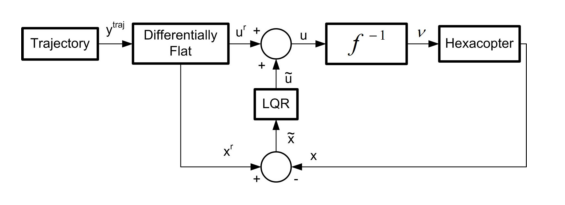
\includegraphics[width=0.7\textwidth]{block_diagram.png}
	\caption{Block Diagram}
	\label{block_diagram}
\end{figure}

Figure \ref{block_diagram} shows the block diagram of the whole system. 

\subsection*{MATLAB simulation}
MATLAB simulation has been developed to verify the feasibility of differential flatness control for multirotor platform. Two trajectories were used: circular trajectory and figure eight trajectory.

\begin{figure}[h!]
	\centering
	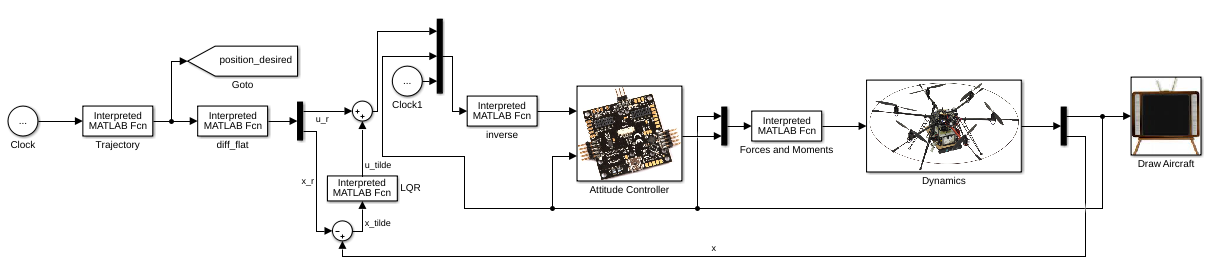
\includegraphics[width=0.7\textwidth]{MATLAB.png}
	\caption{Simulink model for differential flatness control of multirotor}
	\label{MATLAB}
\end{figure}

With the Simulink model shown in the Figure \ref{MATLAB}, Figure \ref{circle} shows the simulated multirotor behavior with circular desired trajectory. Multirotor seems to fly well following circular shape. However, significant steady state error can be observed because the radius of desired circular path is only 5. This initially led to develop integrator augmented LQR controller, but still remains as future work. Figure \ref{eight} shows the simulated eight-figure trajectory following. Trajectory is followed quite well with less steady state error than circular trajectory. Still, adding integrator will be helpful to get closer to the desired trajectory.

\begin{figure}[h!]
	\centering
	\begin{subfigure}{.5\textwidth}
		\centering
		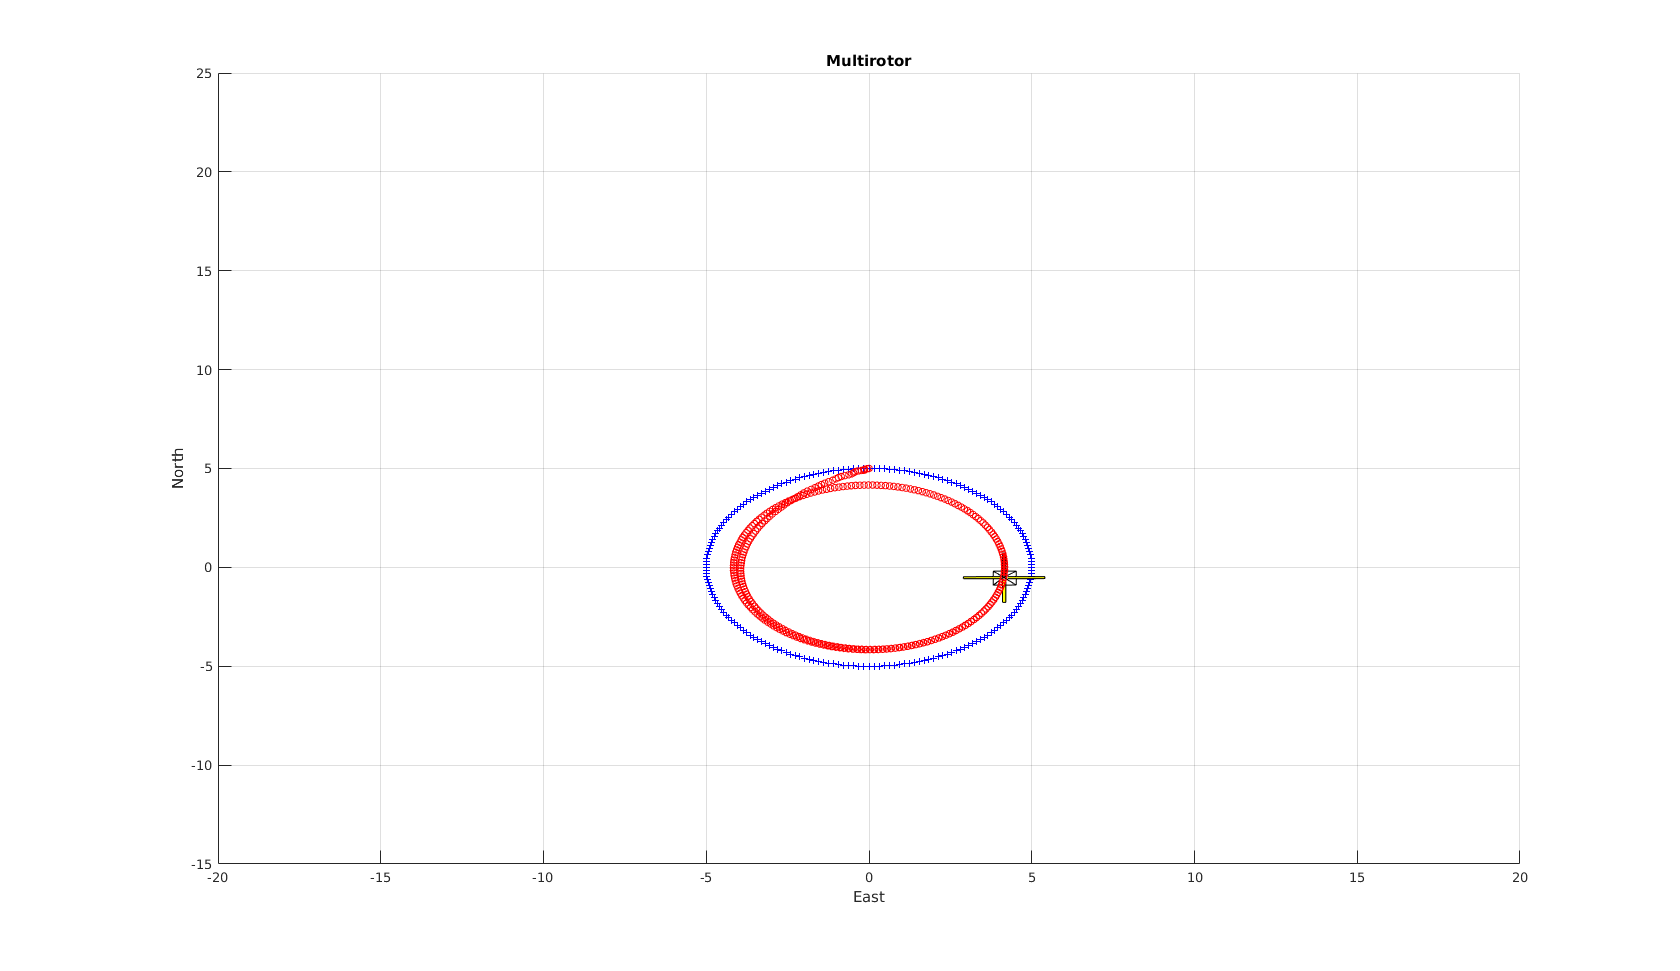
\includegraphics[width=0.9\linewidth]{simulink1.png}
		\caption{Multirotor circular trajectory(Blue: desired trajectory, red: actual trajectory)}
		\label{simulink1}
	\end{subfigure}%
	\begin{subfigure}{.5\textwidth}
		\centering
		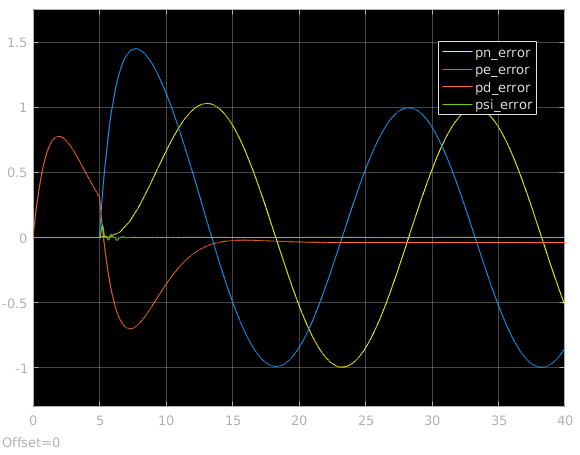
\includegraphics[width=0.7\linewidth]{simulink2.png}
		\caption{Position and heading error}
		\label{simulink2}
	\end{subfigure}
	\caption{Circular trajectory simulated in Simulink}
	\label{circle}
\end{figure}

\begin{figure}[h!]
	\centering
	\begin{subfigure}{.5\textwidth}
		\centering
		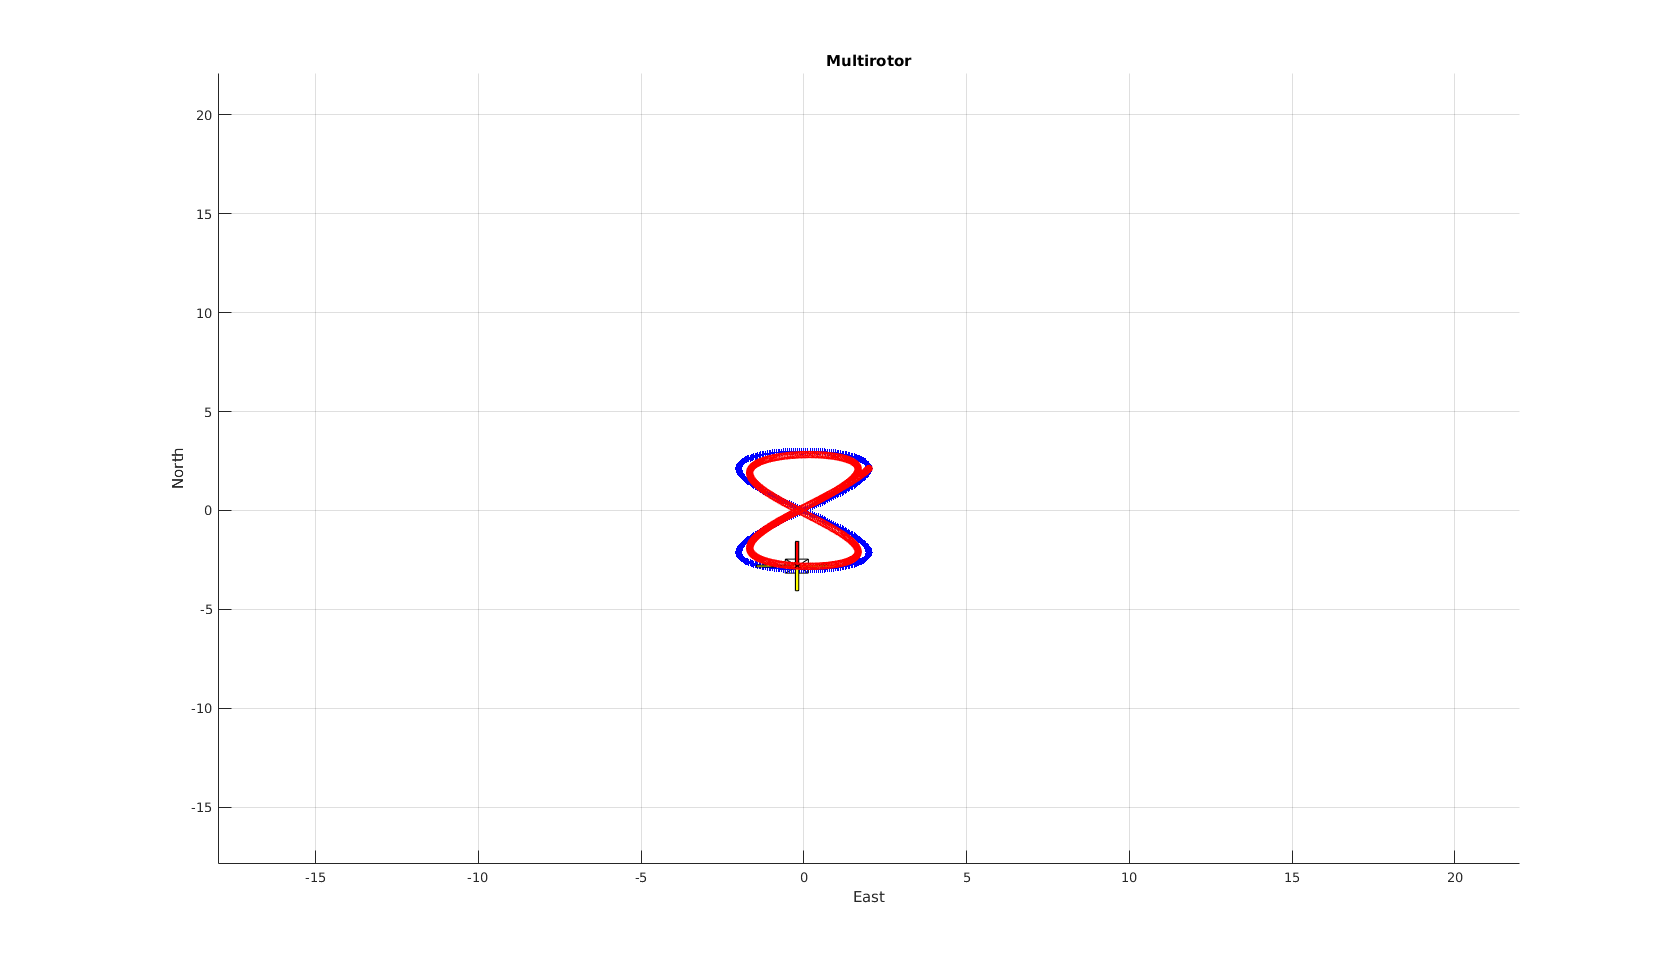
\includegraphics[width=0.9\linewidth]{simulink3.png}
		\caption{Multirotor figure-eight trajectory(Blue: desired trajectory, red: actual trajectory)}
		\label{simulink1}
	\end{subfigure}%
	\begin{subfigure}{.5\textwidth}
		\centering
		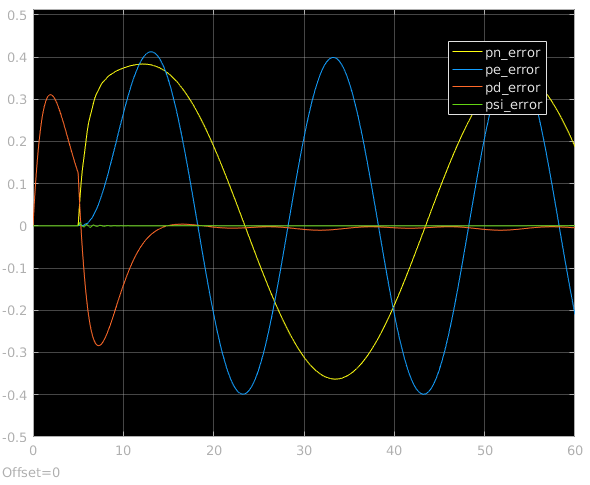
\includegraphics[width=0.7\linewidth]{simulink4.png}
		\caption{Position and heading error}
		\label{simulink2}
	\end{subfigure}
	\caption{Figure-eight trajectory simulated in Simulink}
	\label{eight}
\end{figure}

\subsection*{ROS/Gazebo simulation}
Robot Operating System(ROS) is a dominant framework for robotics programming. It allows robotic system to be modular which makes it clear to users and engineers to see each component and what it is doing. Gazebo is a simulator specifically designed for robotic system. It simulates physics, collision, sensor etc. Since MAGICC lab had a quadrotor simulator in Gazebo that takes thrust, phi, theta, and yaw rate, what had been done in MATLAB was able to tried in Gazebo simulator as well. Only circular trajectory is simulated and the result is comparable with that of MATLAB simulation: circular shape with steady state error.

\begin{figure}[h!]
	\centering
	\begin{subfigure}{.5\textwidth}
		\centering
		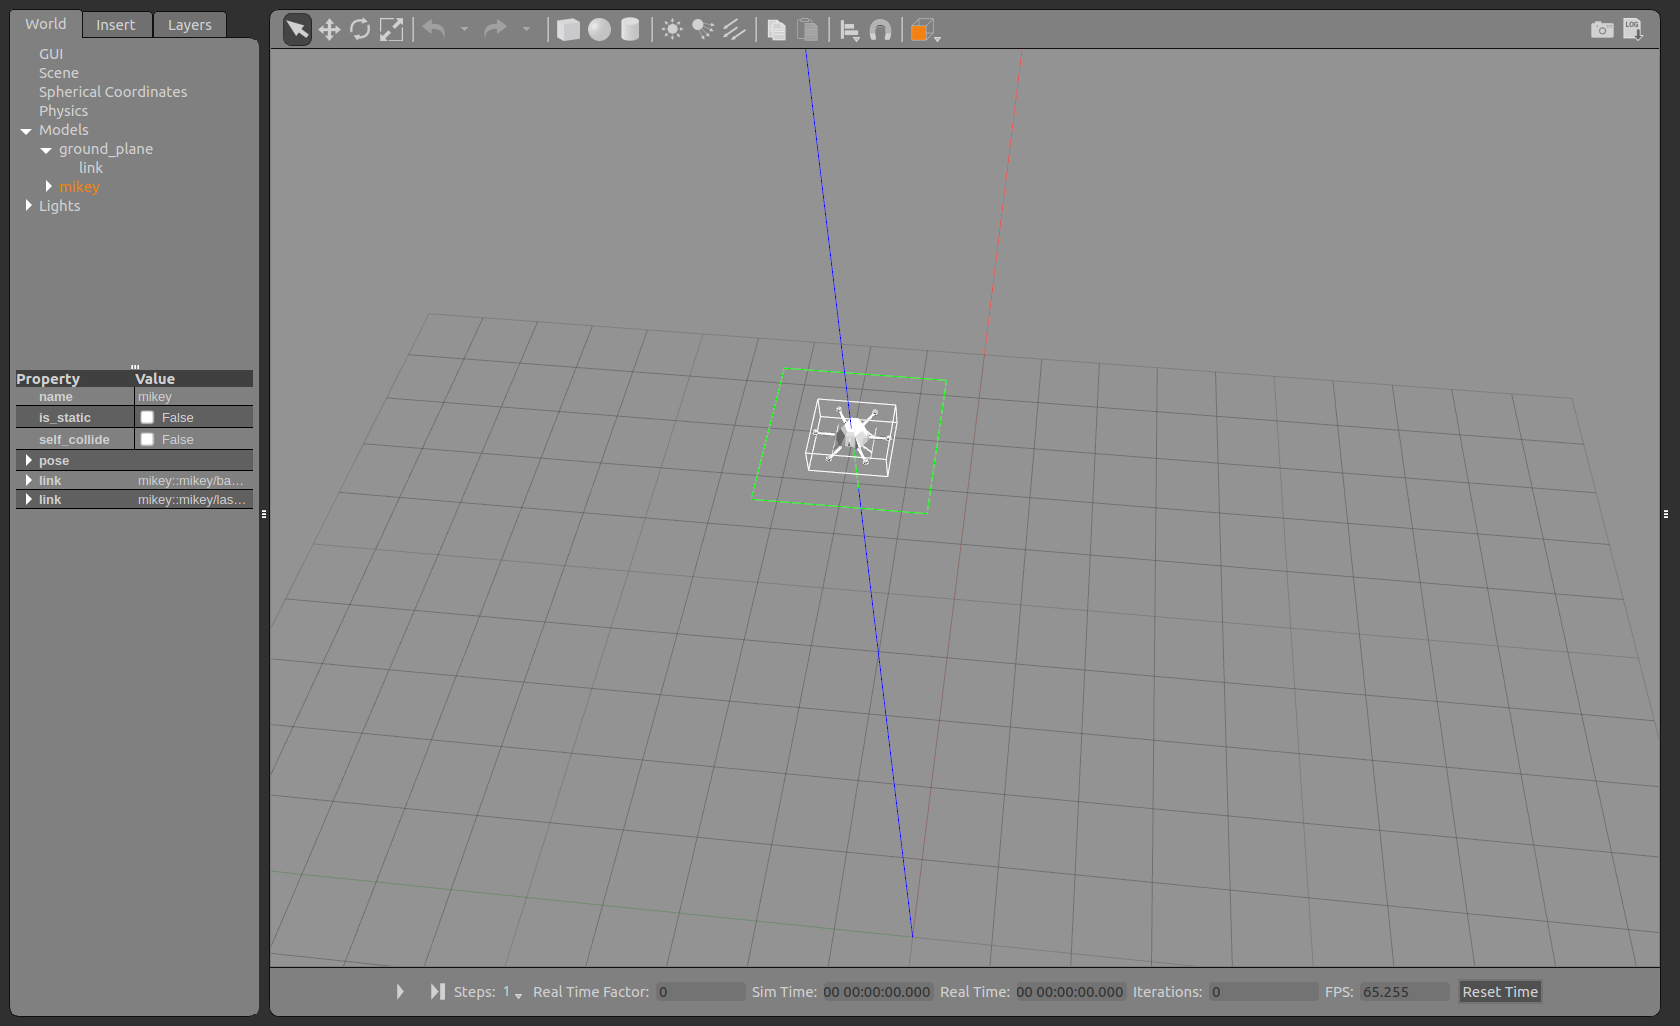
\includegraphics[width=0.9\linewidth]{gazebo1.png}
		\caption{Gazebo multirotor}
		\label{gazebo1}
	\end{subfigure}%
	\begin{subfigure}{.5\textwidth}
		\centering
		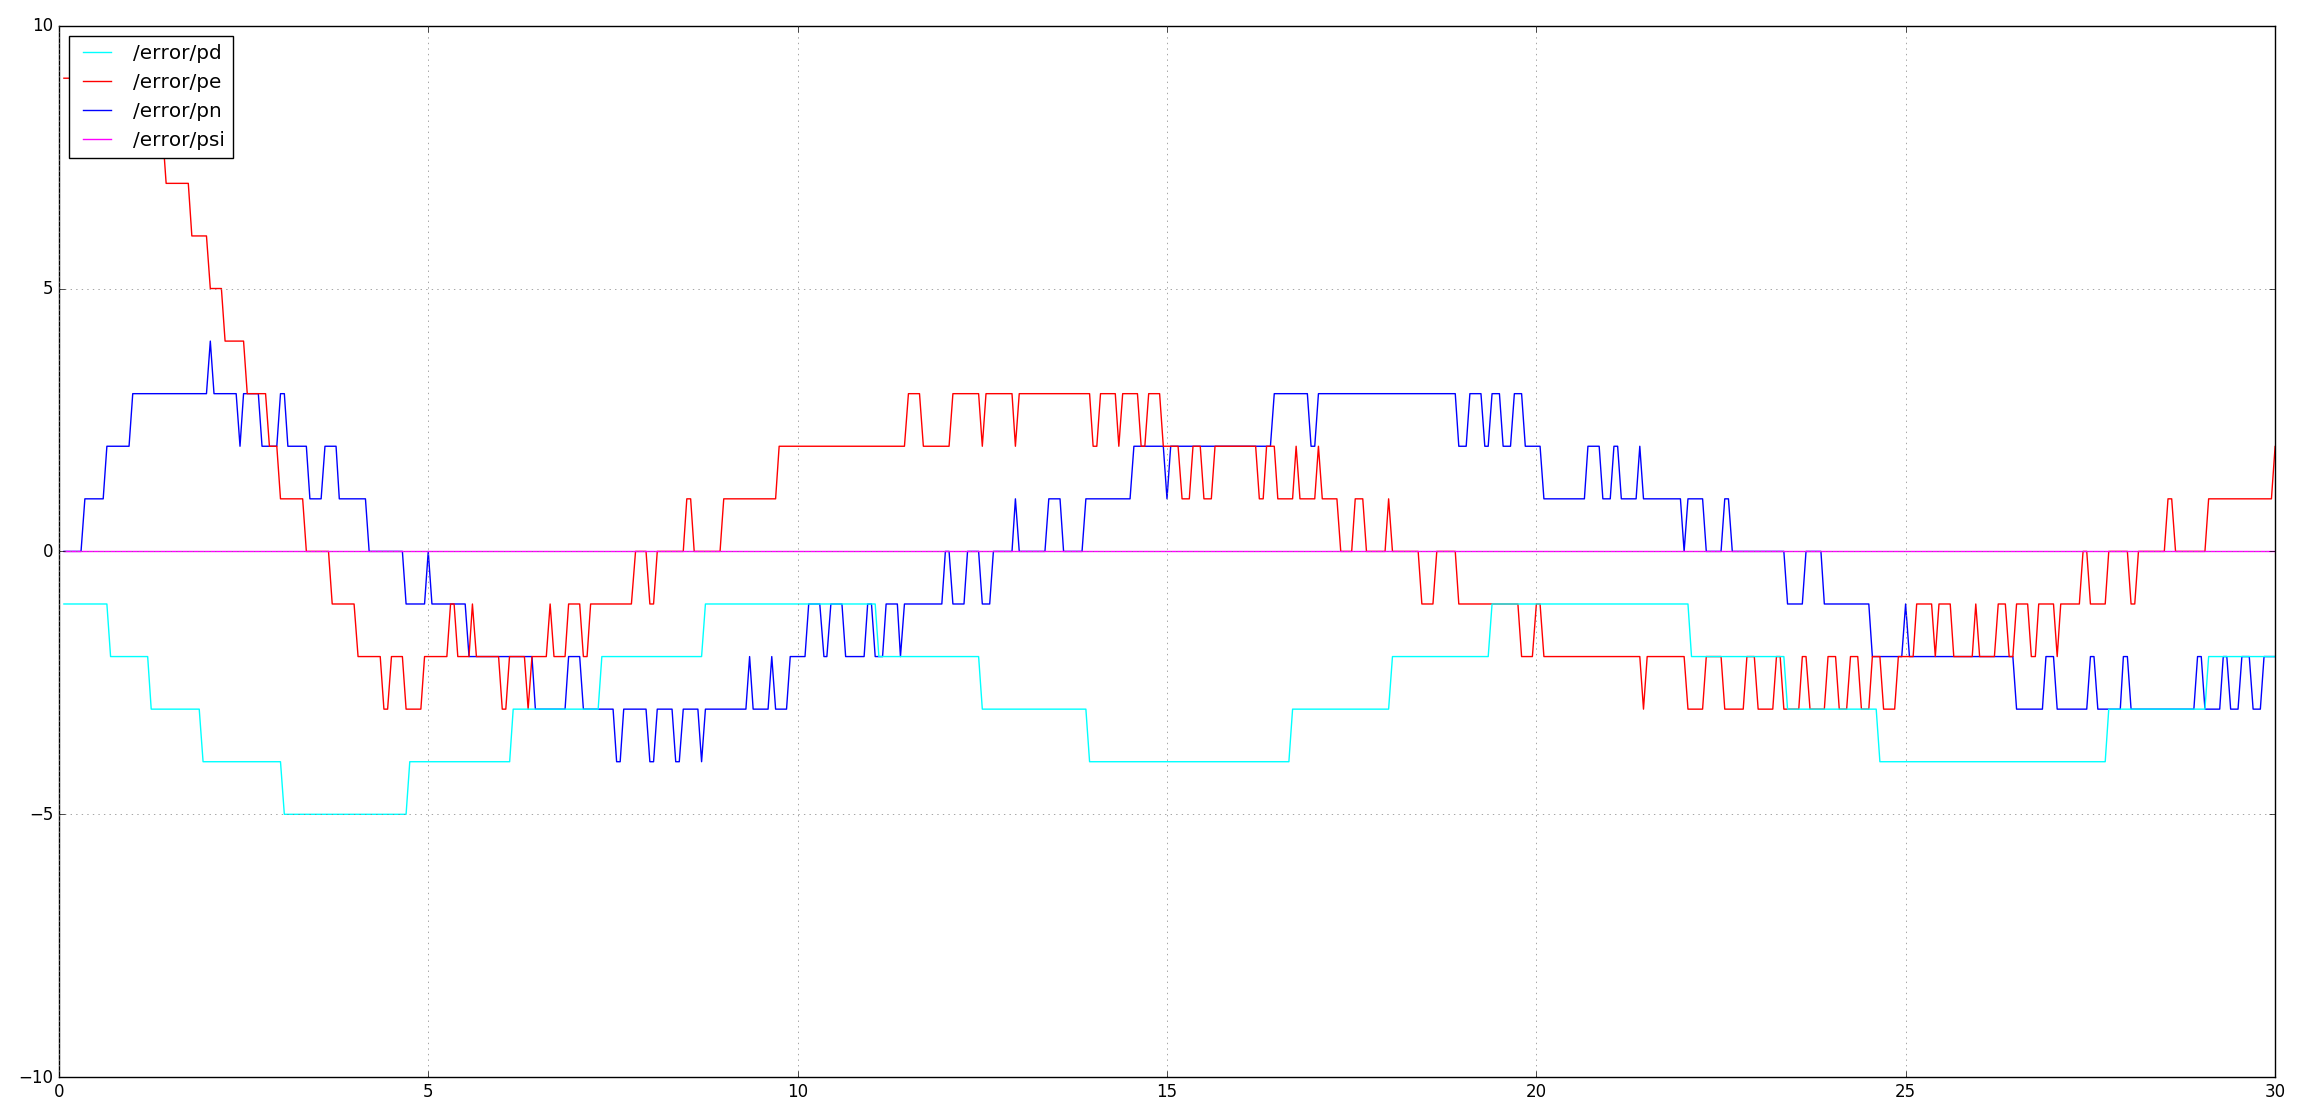
\includegraphics[width=1.0\linewidth]{gazebo2.png}
		\caption{Position and heading error in Gazebo simulator with circular trajectory with radius of 10}
		\label{gazebo2}
	\end{subfigure}
	\caption{Circular trajectory simulated in Gazebo}
	\label{gazebo}
\end{figure}


\subsection*{Conclusion}
Differential flatness control for multirotor has been studied and proved that it can be used as a position and heading controller. MATLAB simulation has been developed to prove the concept and Gazebo simulation has also been developed to fill the gap between MATLAB simulation and real hardware implementation. Developing stable integrator augmented LQR, implementing hardware remain as futurework. 


\begin{thebibliography}{9}
	
[1] J. Ferrin, R. Leishman, R. Beard, and T. Mclain, “Path Planning and Control Utilizing Differential Flatness of Rotorcraft,” vol. 0, no. 3.

\end{thebibliography}

\end{document}